\documentclass[a4paper]{jpconf}
\usepackage{graphicx}
\begin{document}
\title{DBS Query Language}

\author{Anzar Afaq, Vijay Sekhri, Yuyi Guo, Lee Lueking}
\address{Fermilab, Batavia, Illinois, USA}

\author{Valentin Kuznetsov}
%\author{Valentin Kuznetsov, Daniel Riley}
\address{Cornell University, Ithaca, NY 14853, USA}

\begin{abstract}
The CMS experiment has implemented a flexible and 
powerful approach enabling users to find data within 
the CMS physics data catalog. The Dataset Bookkeeping 
Service (DBS) comprises a database and the services 
used to store and access metadata related to its physics 
data. In addition to the existing WEB based and programmatic 
API, a generalized query system has been designed and built. 
This query system has a query language that hides the 
complexity of the underlying database structure. This provides 
a way of querying the system that is straightforward for 
CMS data managers and physicists. The DBS Query Language 
uses the ANTLR tool to build the input query parser and tokenizer, 
then a query builder using a graph representation of the 
DBS schema constructs the actual SQL sent to underlying database. 
We will describe the design of the query system and provide 
details of the language components. We will also provide an 
overview of how this component fits into the overall data 
discovery system, as well as providing access to information 
about Data Quality and Luminosity.
\end{abstract}

\section{Introduction}
In preparation of data taking the CMS experiment at Large
Handron Collider developed very sophisticated set of tools
to collect and bookkeep data effectively. As expected with
start-up of LHC the CMS experiment will produce a few
PB of data each year. Those data will be distributed all
around the world to allow physicists explore a tiny
details of our Universe. In today's environment
a fast, efficient data look-up represents not only a
real challenge but also a key ingredient of successfull
analysis of produced data. In CMS the Data Bookkeeping
system\cite{DBS} is authorative source of information
of meta-data produced by the experiment. It collects
information from broad variety of workflow tools and allow 
physicists to search and look-up their data.

\section{Searching for the tool}
Today there are only two major technologies providing a search capabilities
for end-users. It is relational DBMS and Information retrieval (IR) systems.
Each of them has its own strength and weaknesses. 
We outlined their differences in table \ref{IR_DBMS}.

\begin{table*}[hbt]
\centering
\begin{tabular}{ll}\hline
\hline

IR & DBMS \\
\hline
Imprecise semantics & Precise semantics \\
Keyword search & SQL \\
Unstructured data format & Structured data \\
Read-mostly, add docs occasionally & Expect reasonable number of updates \\
Page through top k-results & Generate full answer \\
\hline
\hline
\end{tabular}
\caption{IR versus DBMS}
\label{IR_DBMS}
\end{table*}

While being designed to address a different domain problems today 
we see that they're become closer to each other. In High Energy Physics (HEP)
domain field such merging becomes more desired with up-coming LHC era.

In HEP the actual data
reside on disk while associative meta-data are stored in databases.
But our users, physicists, wants to look-up data using flexibility of
IR approach and precision of DBMS. By that we mean that providing a {\it Higgs}
keyword is not sufficient for DBMS system to know where to map it. It needs
to be translated to table.column in underlying schema and passed to appropriate
data service.
In addition, our users wants
to search for data using a set of precise conditions and select only those
data which satisfy those criterias. For example, 
{\it I want to find a Higgs sample who was processed with software release
1.2.3 and has runs between 100 and 200}. Obviously such request is
hard to address using IR approach while easier with DBMS. 
Such set of use cases were reviewed by some of us
\cite{DBS07} during development of Data Discovery tool for CMS. We explored
variety of UI's and methods to address those kind of questions. As a
consequences a DBS Query Language (QL) was born. It represents a mixture
of both approaches, IR and DBMS, in a sense that it has precise
semantics of DBMS for data look-up and flexibility of
keyword search as in IR systems.

\section{From SQL to QL}
The growing amount of information stored to DBS system very soon
will represent a challenge for physicists and data managers efficiently
look-up their data. Several user interfaces were proposed to solve this issue.
Among them, structured top-down approach where users look-up their
information from provided list of known entities, such as
trigger line, dataset name, etc.
Even though the web UI
was very intuitive to learn via drop down menus related to each
other, it reaches its limit when the number of entries to look in each menu
becomes significantly large.
Simple management of those lists in a browser represents a real issue and
soon the simplicity of data look-up loose its attraction. By that time
we took orthogonal approach and proposed Query Language (QL) as
a main interface to look-up data in DBS.

DBS QL semantics was kept very close to SQL one. It natuarally
maps into user mental model and was easily adopted by CMS
community. After several iteration we end-up with the following syntax:
\[
find\,\,\,
key_1,\, key_2,\, ...\,\,\, where\,\,\,
\langle key\rangle\, 
\langle op\rangle\, 
\langle value\rangle \,\,\, and|or ...
\label{QL_syntax}
\]
Here $find, where, and, or$ are reserved keywords
which we adopted from SQL syntax\footnote{Except {\it find} special
keyword we used all SQL keywords, e. g. {\it between, in}, etc.}
The keys, both selection and condition ones, were defined
in DBS QL based on slang used by physicists, e.g. dataset, file, run. 
These keys map into internal DB table column or just entire table and 
were structured as entities and their attributes. For example,
a {\it file} refers to file name. At the same time it represents an
entity and maps to file table. Obviously such table
contain more information about the files, such as their size, creation time,
type etc. This information were referred as a file attributes, e.g.
{\it file.size, file.createdate, file.type}. Some of the attributes
where presented for all QL keys, e. g. {\it createdate, createby}, etc.,
while others were only unique to certain entities, e.g. {\it release.family}.

To accomodate flexibility of searching criterias DBS QL supported a
broad variety of boolean operators, such as $>, >=, <, <=, =, like$, etc.,
see $\langle op\rangle$ in \ref{QL_syntax}. Basically,
since we map our QL expression to SQL, our limitation were based
on SQL one. A complex expressions were very well adopted via
usage of brackets and combination of constrains.

The figure \ref{Grammar} represents a simplified view of the grammar
that defined the semantics of the DBS QL.
\begin{figure}[htb]
\centering
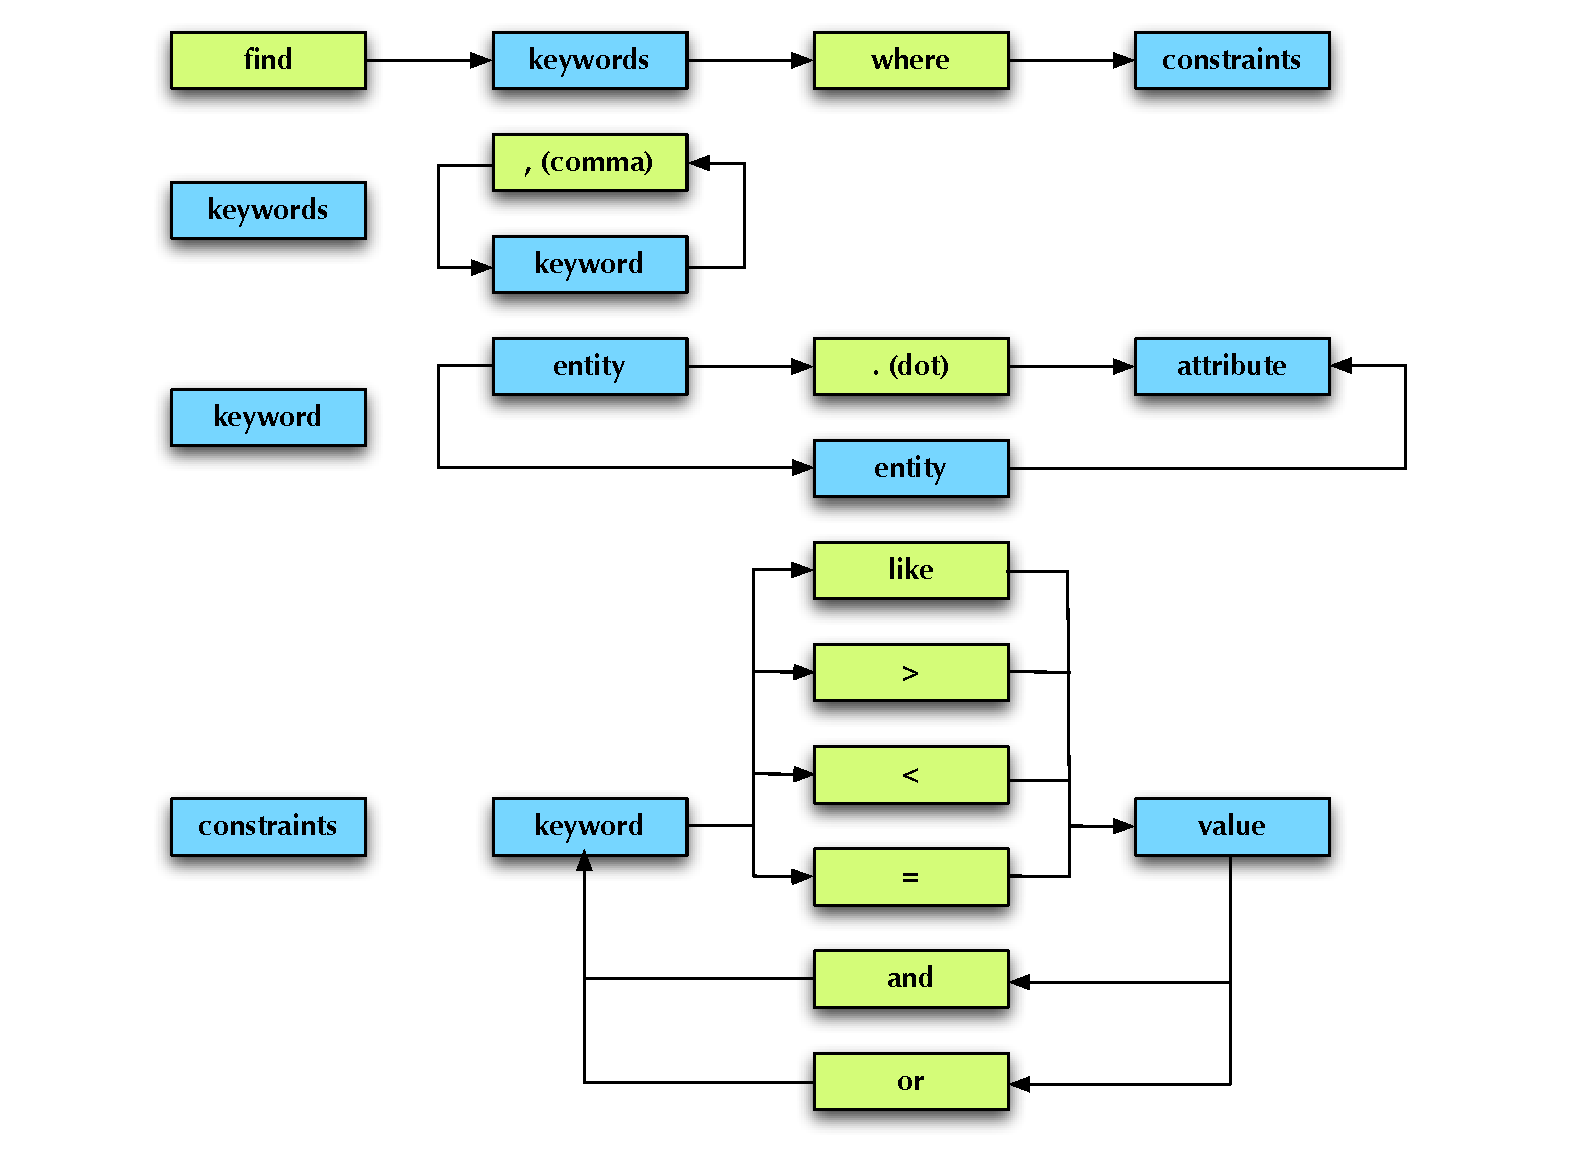
\includegraphics[width=150mm]{DBSSql_grammar.pdf}
\caption{
DBS QL grammar.
}
\label{Grammar}
\end{figure}
In this diagram the entities (keys) are represent logical tables. 
Each entity has a set of additional attributes (table’s columns). 
The grammar allows any combination of 
attribute and entity, however not every attribute
is appropriate for each entity. An incorrect
combination was detected by the Query Builder at run time
and appropriate message was provided to end-user with
precise position of the error. The aggregation functions, such
as sum, count where added to the grammar as well. 

Such semantics gave us a great felxibility to construct
arbitrary queries against DBS using published DBS QL keys.
To achieve that we defined external mapping between
tables and a graph nodes and 
Dijkstra’s shortest path algorithm to find a join conditions
for provided user query.

\section{DBS QL architecture}

The DBS code used a well known 3-tier architecture. The server
code was developed using Java Servlets placed into tomcat container.
Its details has been discussed elsewhere\cite{DBS} and we will skip
them here. 

The DBS QL was originally prototyped in Python and then implemented
in Java using ANTRL tool. Its architecture is shown on Fig. \ref{DBS_QL}.
\begin{figure}[htb]
\centering
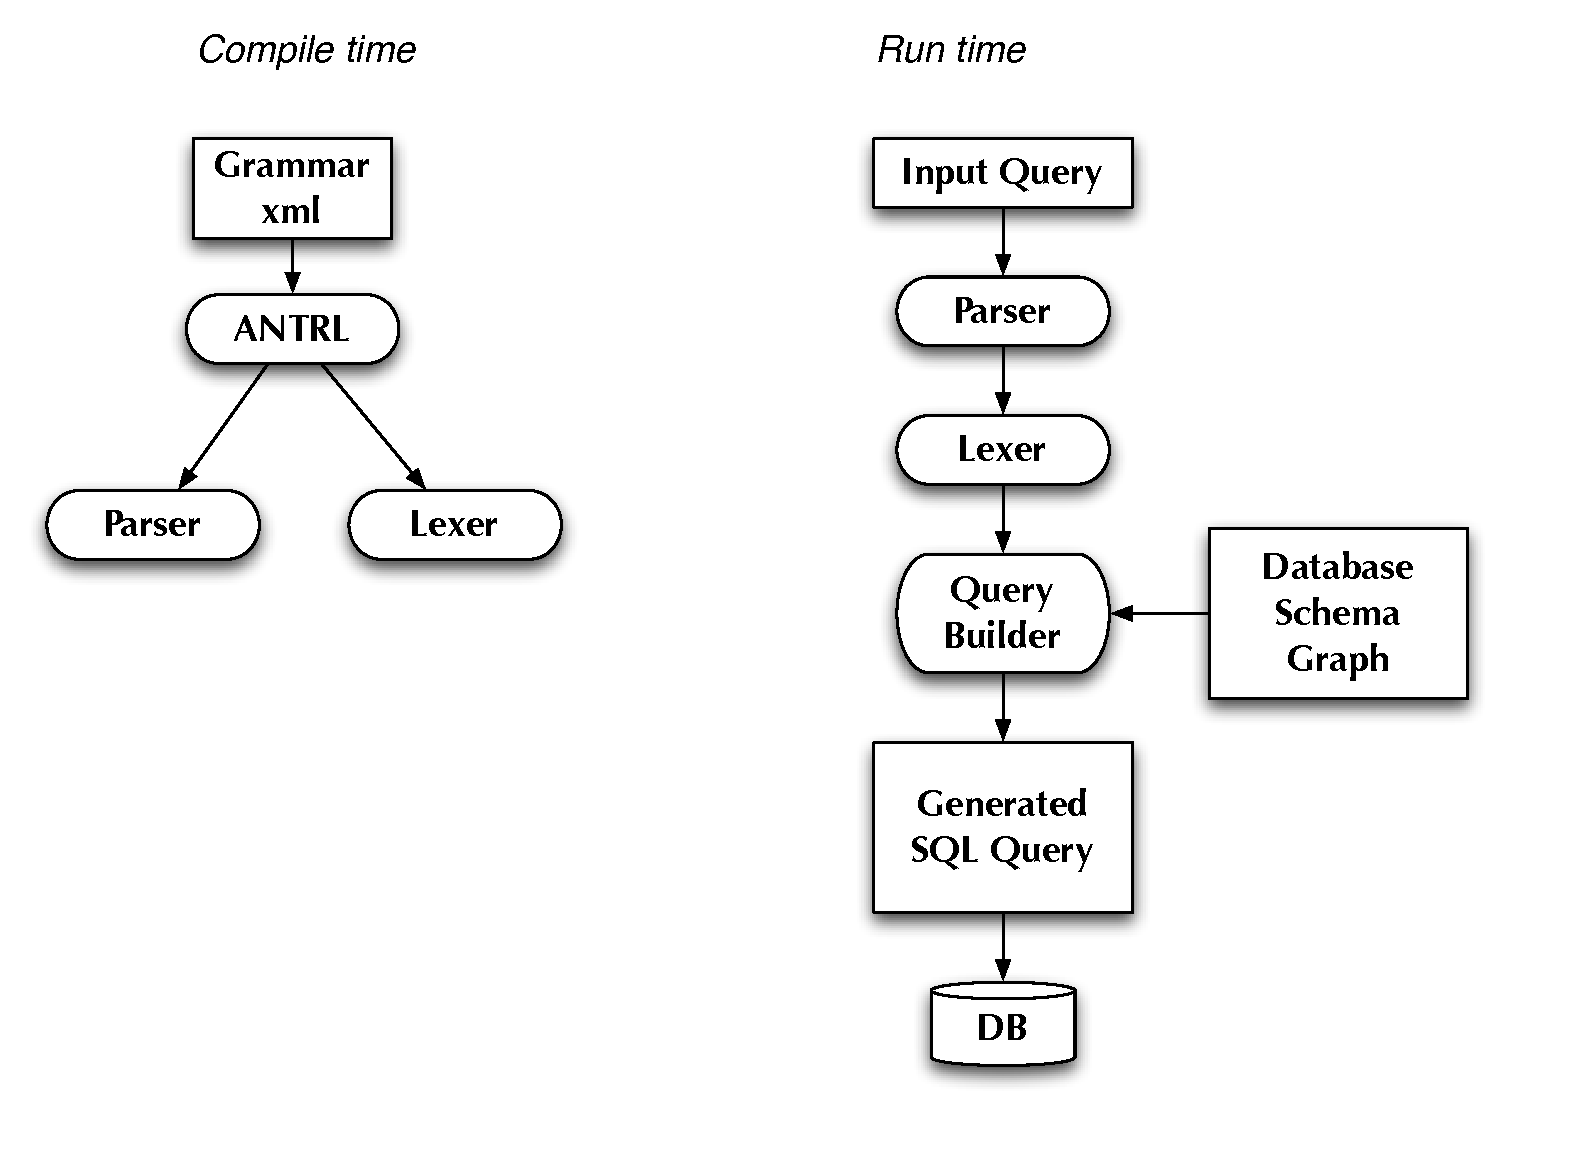
\includegraphics[width=100mm]{DBS_QL_architecture.pdf}
\caption{DBS QL architecture.}
\label{DBS_QL}
\end{figure}
It was divided into two parts. A static generation of DBS QL
parser and lexer by using grammar file and ANTLR tool\cite{ANTLR}
and generation of the SQL query at run time out of provided user query.

Regarless of UI (web or command-line), the user query was 
passed to the server where it was interpreted by a lexer and a parser.
Then the Query Builder generates a valid SQL query suitable for
execution at DB back-end.\footnote{We officially supported ORACLE and
MySQL back-ends.} 
The ANTLR tool was used an external grammar file which defined 
the syntax and semantics of DBS QL. It generated the parser and lexer 
code for compile time. Therefore a new addition to QL, such as key,
attribute and/or support for boolean expression, had a drawback of
regenerating the parser and lexer code and its redeployment on a server.
 
The entire database schema was represented as a weighted
directed graph with nodes mapped to tables, and edges 
representing relationships between tables. The Query Builder
used the Dijkstra’s shortest path algorithm to determine a 
path from one table to another and resolve multi-path ambiguities.
The chosen path is used to construct the final SQL query. 
For example, the Fig. \ref{ShortestPath} shows database tables 
T1 through T4  where edges between the tables represents the 
relationships between the tables.

\begin{figure}[htb]
\centering
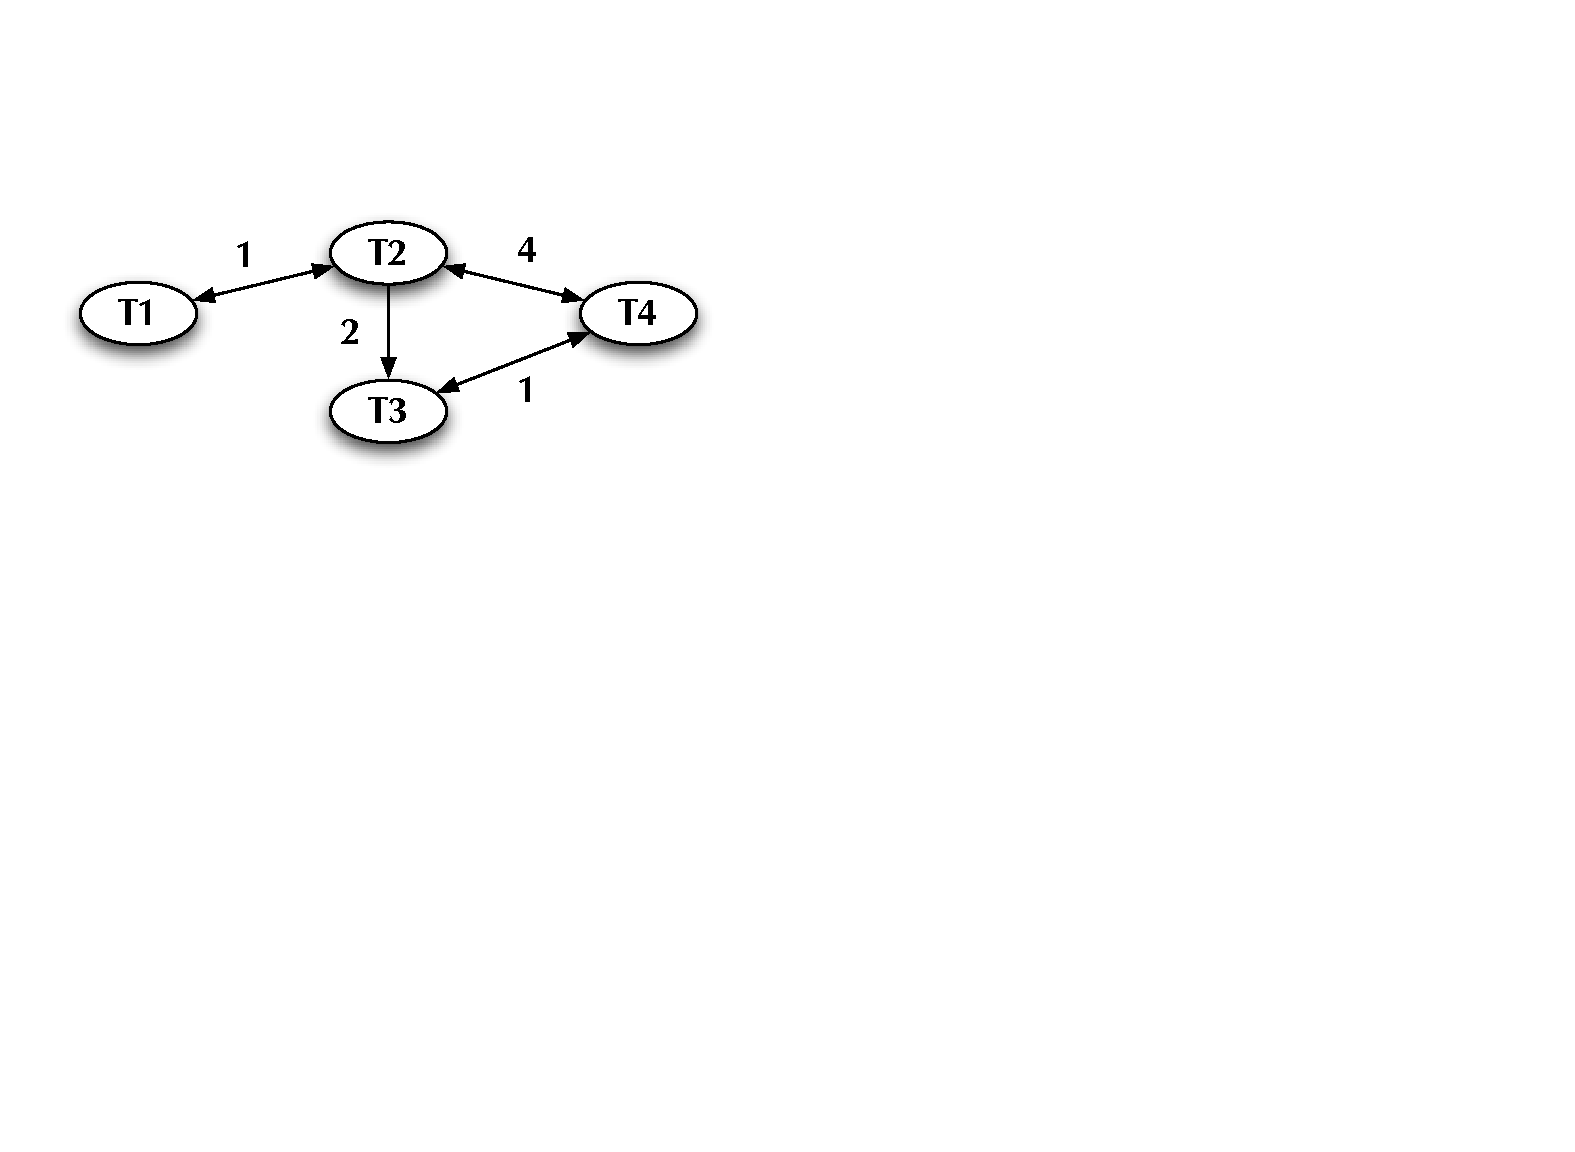
\includegraphics[width=80mm]{DBSSql_shortestpath.pdf}
\caption{A graph which represents different paths between tables. The
numbers are weigths assigned to each table such that a shortest path
can be computed. For example, the shortest path from table T1 to T4 is 
T1 $\rightarrow$ T2 $\rightarrow$ T3 $\rightarrow$ T4 with total weight 
equal 4. While the shortest path from table T4 to T1 is 
T4 $\rightarrow$ T2 $\rightarrow$ T1, due to prohibited path
between T2 and T3, with total weight of 5. 
}
\label{ShortestPath}
\end{figure}
If any ambiguity has happened between 2 or more paths, i.e.
their total weight was calculated to be the same, we manually 
resolved it based on concrete use case. 
Such resolution was done in external schema graph file.

Since DBS QL hided all relationship among tables and didn't
expose the actual table names, the users were allowed to
select any key, key.attribute combinations in their queries.
Those were mapped back to table, table.columns, such that
Query Builder was able to find a shortest path
from one table to another without specifying intermediate
tables and join conditions.
In this forementioned example \ref{ShortestPath},
if user specified
$
find\,\, key_1, key_4\,\, where\,\, ...
$
and $key_1, key_4$ maps into T1 table and T4 tables respectively,
the Query Builder determines
the shortest path 
T1$\rightarrow$T2$\rightarrow$T3$\rightarrow$T4 
and added the intermediate tables 
and the join conditions to the final SQL query. 

It is worthwhile to mention that DBS QL can be adopted to
any DB schema, using any DB back-end and programming interface.
It provides additional mapping between your data model and
user interface by making a bridge between user mental model
and relational model of your data. Such mapping is important
to allow users place their queries without any knowledge of
underlying data model. 
In fact, as will be discussed in
next section, we currently exploring a possiblity to
expand DBS QL to other data services and combine them
into a single aggregation layer for end-users.

\section{DBS QL intergration with CMS tools}
Very soon the DBS QL becomes a language of choice to search
and look-up data in CMS. Due to simple web interface of
Data Discovery\cite{DD}  and its integration with DBS QL
users were able to find their data quickly and very
efficiently. Over time the Data Discovery UI has
change several times, from menu-driven approach using
direct connection to DB to DBS QL presentation layer
using stateless connection to any DBS instances deployed
within CMS. Our users started adopting DBS QL in their
own applications, performing monitoring of their
site usage, customizing views for data-centers
and developing easy to use data-services, such as
FileMover\cite{FileMover}. To demonstrate both simplicity,
flexibility of DBS QL here is a simple, but realistic,
code snippet in python which query run summary information
for given dataset
\begin{verbatim}
import urllib, urllib2

dbsurl = "http://host/DBSServlet"
query  = "find run, run.numevents, count(files) where dataset=/a/b/c"
params = {'apiversion':'DBS_2_0_6','api':'executeQuery', 'query': query} 
data=urllib2.urlopen(dbsurl,
             urllib.urlencode(params,doseq=True)).read()
result = data.read()
\end{verbatim}
Along with Data Discovery web interface the DBS itself 
provided a simple stand-alone command line tool
to search data from a fingertips of the users in their
favorite environment. This tool was written
in python, doesn't require any dependencies and can
be used on any OSes within CMS community.

Moreover, DBS QL simplicity force us to explore a further
extentions of QL to other data-services deployed in CMS under
the umbrella of Data Aggregation Service (DAS). The DAS idea is
novel within CMS and still under development.
It allows users to place query across multiple data-services,
such as DBS, SiteDB, PhEDEx, Luminosity DB, etc. Its semantic
is based on DBS QL one and naturally
expand boundaries of later to other services providing
end-users a reach set of flexible keys to be used in their
queries. But instead of mapping DAS QL into a single
schema, we exploring how to map it to data-service APIs. 

\section{Summary}
We discussed a novel approach of searching data within CMS
collaboration. It is based on flexible,
intuitive and expandable query language using
semantics of mental model of physicsists used in their 
daily operations.
By hiding relationships and mapping well-known
keys and their attributes to underlying data-service
schema we achieve a scalable power of QL. Its utilization
were well adopted in CMS via web interface and widely
expanded in various workflow and analysis tools. Physicists
were able to quickly answer their questions about data by
speficying selection keys and providing set of conditions
in their user query. We demostrated that such approach
can be adopted to any DB schema and can be implemented
in any language.

\section{Acknowledgements}

This work was supported by National Science Foundation.

\section*{References}
\begin{thebibliography}{9}
\bibitem{DBS} A. Afaq, et. al. ``The CMS Dataset Bookkeeping Service'', CHEP 2007 
\bibitem{DBS07} A. Dolgert, V. Kuznetsov, C. Jones, D. Riley, 
``A multi-dimensional view on information retrieval of CMS data'', CHEP 2007
\bibitem{DD} https://cmsweb.cern.ch/dbs\_discovery
\bibitem{ANTLR} http://www.antlr.org
\bibitem{FileMover} B. Bockelman, V. Kuznetsov ``CMS FileMover: one click data'', CHEP 2009

\end{thebibliography}

\end{document}


